\documentclass{article} 
\usepackage{tikz} 
\begin{document} 
\begin{tikzpicture}[node distance={22mm}, thick, main/.style = {draw, circle(15mm)}]
\node[main] (1) {$love_01$}; 
\node[main] (2) [below right of=1] {$x$};
\node[main] (3) [below left of=1] {$y$}; 
\draw[->] (1) -- node[midway, above right, sloped, pos=1] {Arg0}  (3);
\draw[->] (1) -- node[midway, above left, sloped, pos=1] {Arg1}  (2);
\end{tikzpicture} 

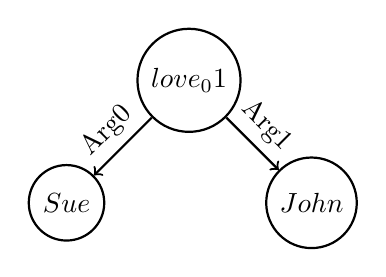
\begin{tikzpicture}[node distance={22mm}, thick, main/.style = {draw, circle}]
\node[main] (1) {$love_01$}; 
\node[main] (2) [below right of=1] {$John$};
\node[main] (3) [below left of=1] {$Sue$}; 
\draw[->] (1) -- node[midway, above right, sloped, pos=1] {Arg0}  (3);
\draw[->] (1) -- node[midway, above left, sloped, pos=1] {Arg1}  (2);
\end{tikzpicture} 
\end{document}